\documentclass{report}

\usepackage{blindtext}
\usepackage{graphicx}
\usepackage{caption}
\usepackage{subcaption}
\usepackage[margin=0.5in]{geometry}

\graphicspath{ {./images/} }

\author{Oskar Mampe: 201368087}
\date{\today}
\title{Convolutional Neural Networks}

\begin{document}
    \maketitle
    \tableofcontents

    \section{Part I: Experimenting with Features}


    Firstly, for my experiments, I have tested various number of layers to see how it affects the performance of the network. I have also decided to validate the performance of different filter size's of the two proceeding convolutional layers.  I have decided to choose different kernel size, the difference being ....

    % Separate the discussion of training and performance. In effect on training, only discuss the perofrmance of the train, the speed and so on. Performance should be about accuracy.
    \subsection{Effect on Training}
    Lower number of layers/kernel influences the speed in which it trains.


    \subsection{Effect on Performance}
    The different models, performed differently, specificly, the lower the number of layers, the more likely it is that the model overfits. This can be seen in the 2 layers model, where the model performed extremely well on the training data, reaching accuracy of 80. However, when the same model was checked against validation and test data, the results were astonoshingly different. The results dropped down to around 40\% on unseen data.

    \begin{figure}[h!]
        \centering
        \begin{subfigure}[t]{0.45\textwidth}
            \centering
            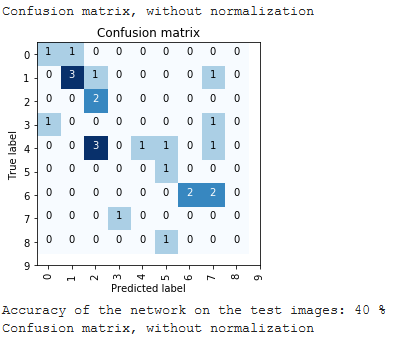
\includegraphics[width=0.5\textwidth]{2_layers}
            \caption{2 Layer Network}
        \end{subfigure}
        \begin{subfigure}[t]{0.45\textwidth}
            \centering
            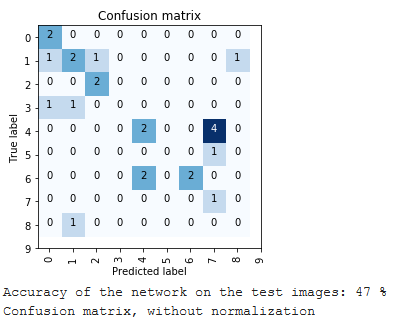
\includegraphics[width=0.5\textwidth]{3_layers}
            \caption{3 Layer Network}
        \end{subfigure}
        \begin{subfigure}[t]{0.45\textwidth}
            \centering
            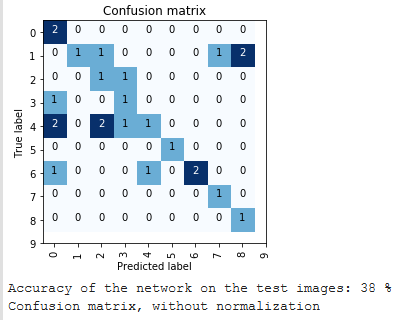
\includegraphics[width=0.5\textwidth]{4_layers}
            \caption{4 Layer Network}
        \end{subfigure}
        \begin{subfigure}[t]{0.45\textwidth}
            \centering
            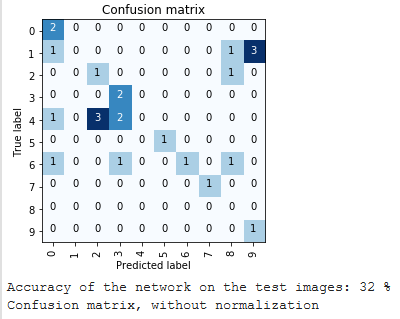
\includegraphics[width=0.5\textwidth]{5_layers}
            \caption{5 Layer Network}
        \end{subfigure}
        \caption{Confusion Matrices for the Different Layers}
    \end{figure}

    As you can see, the layers perform better with a lower number of layers, the sweet spot being around 3.
    \begin{figure}[h!]
        \centering
        \begin{subfigure}[t]{0.45\textwidth}
            \centering
            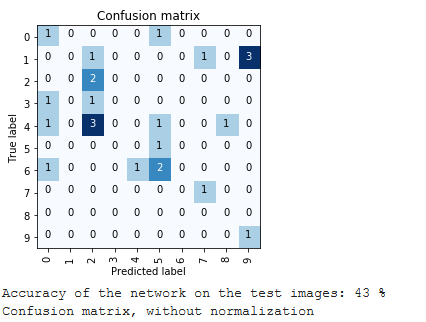
\includegraphics[width=0.5\textwidth]{2_ks}
            \caption{2 Filter Size Network}
        \end{subfigure}
        \begin{subfigure}[t]{0.45\textwidth}
            \centering
            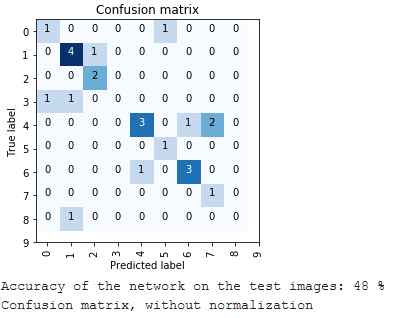
\includegraphics[width=0.5\textwidth]{3_ks}
            \caption{3 Filter Size Network}
        \end{subfigure}
        \begin{subfigure}[t]{0.45\textwidth}
            \centering
            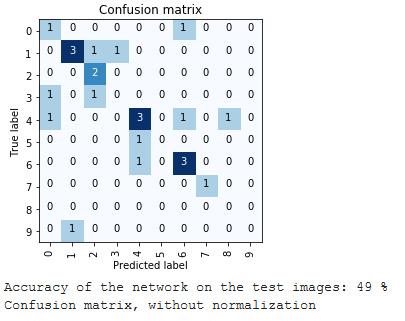
\includegraphics[width=0.5\textwidth]{4_ks}
            \caption{4 Filter Size Network}
        \end{subfigure}
        \begin{subfigure}[t]{0.45\textwidth}
            \centering
            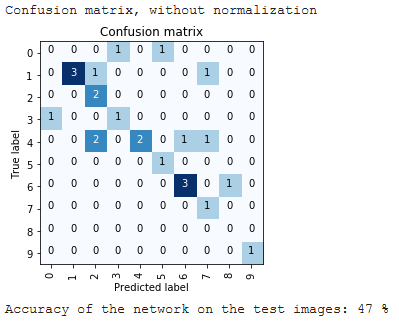
\includegraphics[width=0.5\textwidth]{5_ks}
            \caption{5 Filter Size Network}
        \end{subfigure}
        \caption{Confusion Matrices for the Different Layers}
    \end{figure}


    \section{Part II: Visualising Filters}

    \subsection{Implementation}

    \subsection{Results}

    \subsection{Comment on the evolution of the filters}

    The 3 channel RGB is further generalised to different features.

    \section{Part III: Visualising Features}
    
    \subsection{Implementation}

    \subsection{Results}

    \subsection{Comment on the evolution of the features}

    \section{Part IV: Experimenting with Network}

    \subsection{Intro}

    \subsection{Change 1: }

    \subsubsection{Motivation}

    \subsubsection{Results}

    \subsection{Change 1: }

    \subsubsection{Motivation}

    \subsubsection{Results}

    \subsection{Change 1: }

    \subsubsection{Motivation}

    \subsubsection{Results}

\end{document}